\documentclass[t]{beamer}


\usepackage[T1]{fontenc}
\usepackage[utf8]{inputenc}
\usepackage[ngerman]{babel}
\usepackage{graphicx}
\usepackage{color}
\usepackage{import}
\newcommand{\themepath}{../latex_templates/theme/}
\subimport{\themepath}{beamerthemefablab-4-3.sty}

\usepackage[font=large,labelfont=bf]{caption}

% Zwei Bilder nebeneinander, gleich hoch
\newcommand{\zweibilder}[3][0.55\textheight]{%
    \begin{center}
        \includegraphics[height=#1,width=0.48\textwidth,keepaspectratio]{#2}\hfill
        \includegraphics[height=#1,width=0.48\textwidth,keepaspectratio]{#3}
    \end{center}
}

\begin{document}
% Title page


\date{\today}
\institute{FAU FabLab}
\title[Mathe-Rep]{Das FAU FabLab}
\author{} % TODO Namen der Vorstellenden eintragen
\frame[plain,c]{\titlepage} % plain-Option deaktiviert Kopf- und Fusszeile


\begin{frame}
    \frametitle{FabLab? Offene Werkstatt}
    % - auf der ganzen Welt
    % - MIT, Prof. Neil Gershenfeld
    % - jede Möglichkeit, kreativ
    \begin{itemize}
        \item \textbf{Weltweit} über 500
        \item Ideen und Wissen miteinander teilen
    \end{itemize}

    \bigskip
    \begin{columns}[c]
        \begin{column}{0.55\textwidth}
            \textit{\glqq In a way, the FabLabs are havens for inventive outliers in society.\grqq}

            \medskip
            {\fontsize{16}{20}\selectfont Prof. Neil Gershenfeld (MIT)}
        \end{column}
        \begin{column}{0.4\textwidth}
            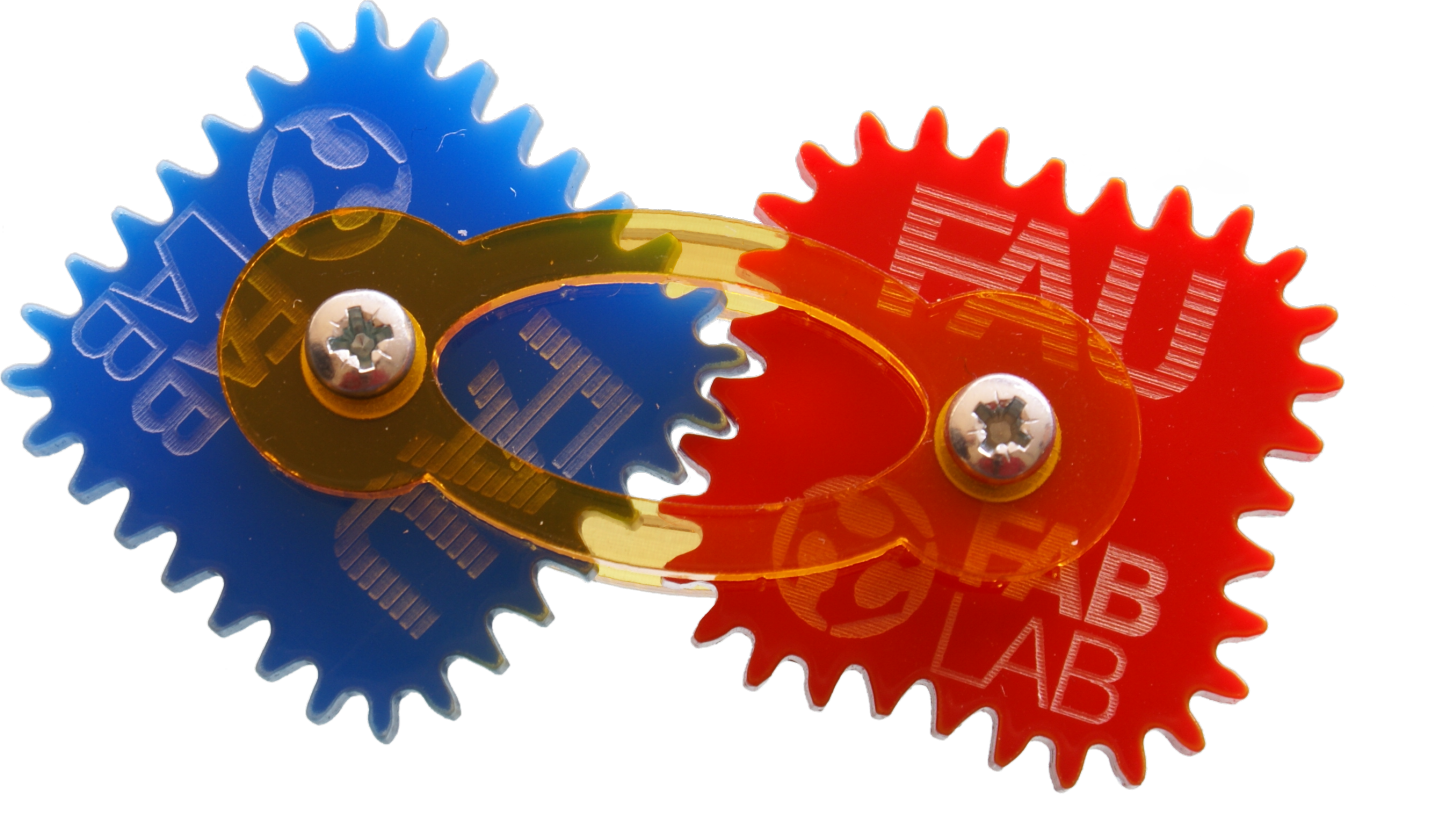
\includegraphics[width=\textwidth]{../img/zahnraeder.png}
        \end{column}
    \end{columns}
\end{frame}

\begin{frame}
    \frametitle{FAU FabLab? Hightech-Werkstatt an der TechFak}
    % - von Studierenden, Ehrenamtliche
    % - für alle
    % - Einweisungen, dann selber machen
    \begin{itemize}
        \item \textbf{Selbständig} Ideen verwirklichen
        \item Lernen, wie's geht
        \item Zum \textbf{Selbstkostenpreis}
    \end{itemize}
    \begin{center}
        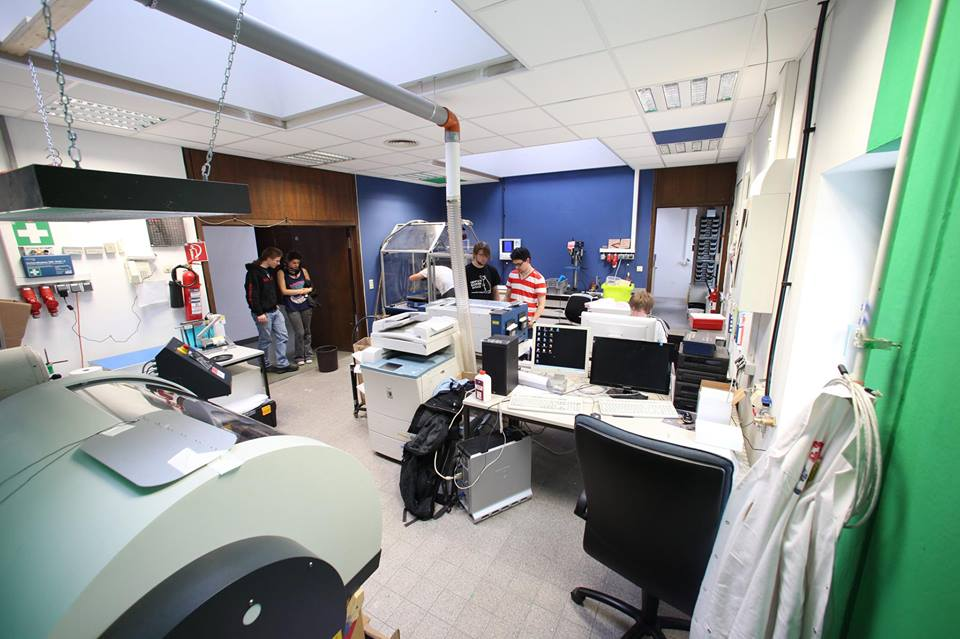
\includegraphics[height=0.5\textheight,width=\textwidth,keepaspectratio]{../img/fablab_fischauge.jpg}
    \end{center}
\end{frame}

\begin{frame}
    \frametitle{Lasercutter}
    % - 100 Watt
    % - schneidet Acryl, Holz, ...; graviert auch Glas, Metalle, ...
    % - Witz: FAU Card
    % - Material ist vorrätig
    \begin{itemize}
        \item Schneidet und graviert
        \item Acryl, Holz, Aluminium
    \end{itemize}
    \zweibilder{../img/mann_am_laser.jpg}{../img/laser_beam.jpg}
\end{frame}

\begin{frame}
    \frametitle{3D-Drucker}
    % - bekannt
    % - mehrere Drucker
    Rapid Prototyping zum Zuschauen
    \begin{center}
        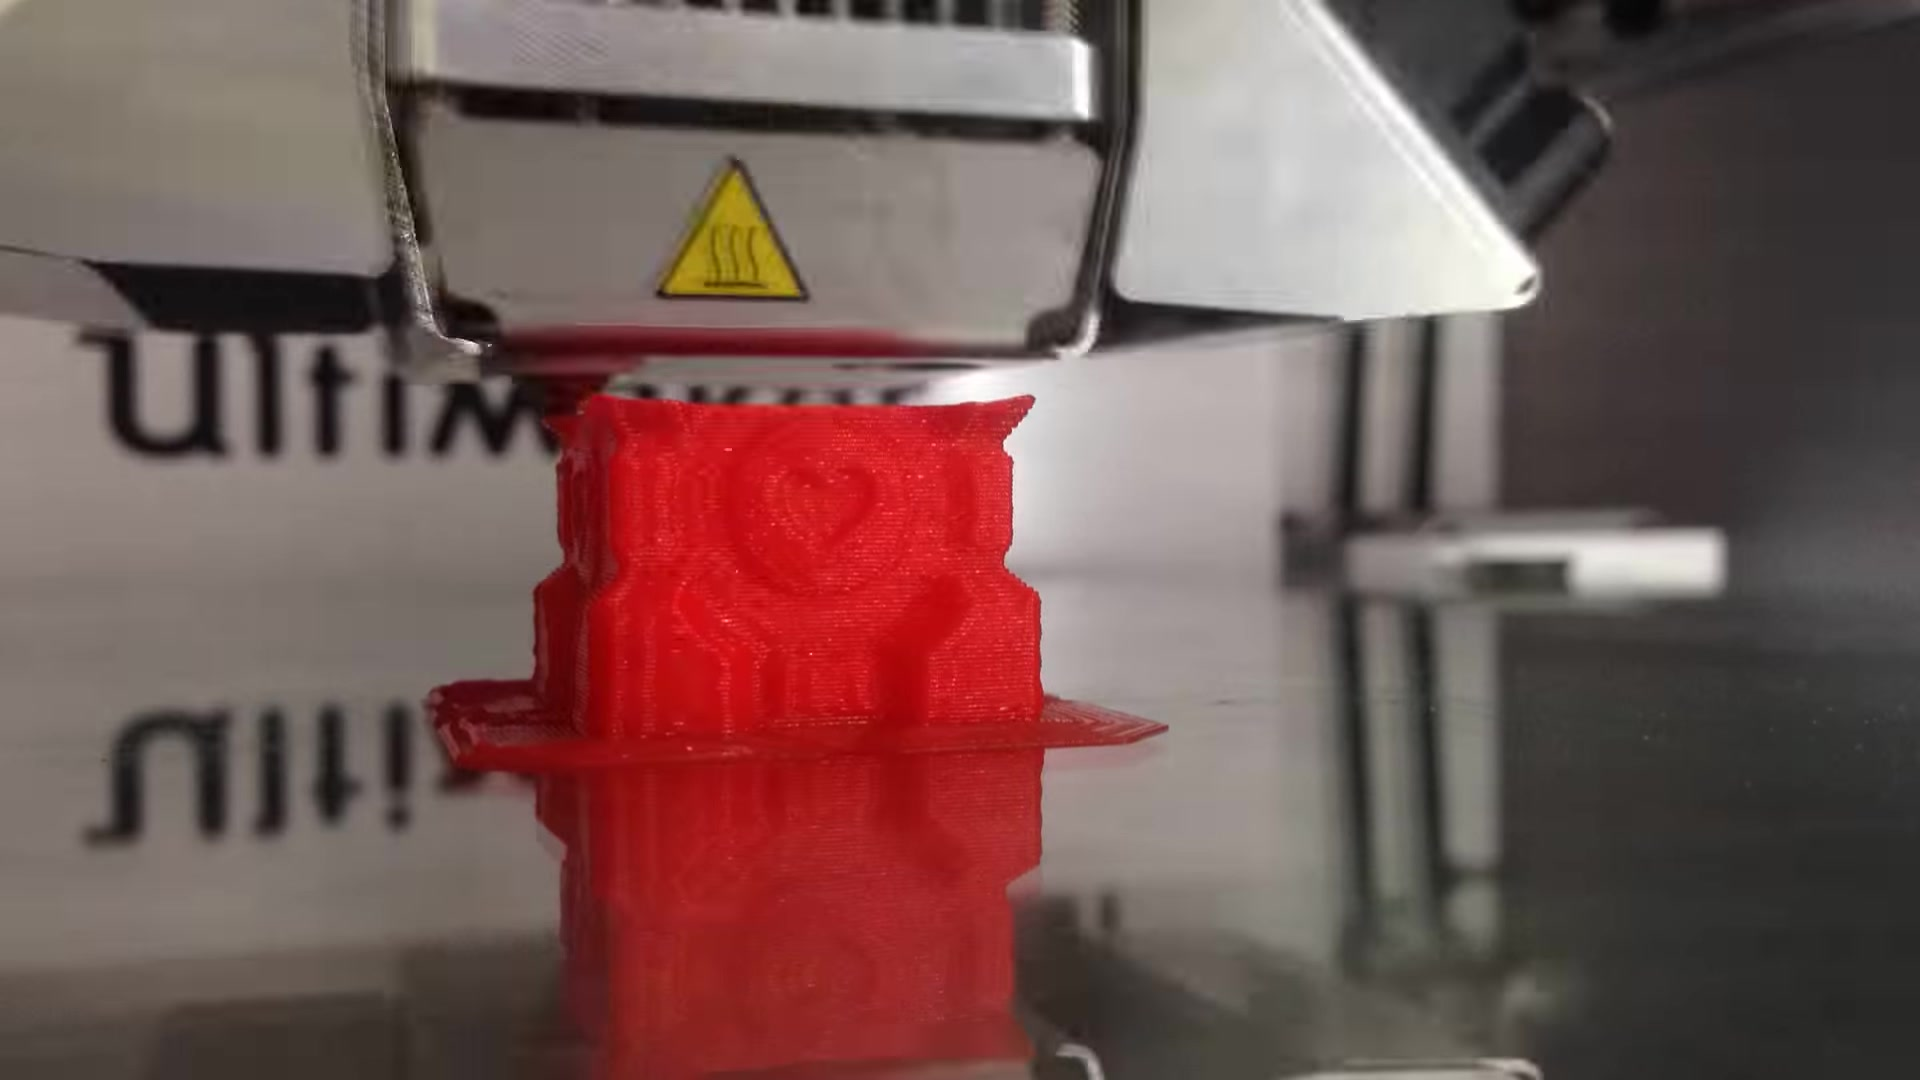
\includegraphics[height=0.6\textheight,width=\textwidth,keepaspectratio]{../img/3d-drucker.jpg}
    \end{center}
\end{frame}

\begin{frame}
    \frametitle{Schneideplotter, T-Shirts}
    % - Folien schneiden, einfach
    % - T-Shirts mit der Presse
    \bigskip
    \zweibilder[0.6\textheight]{../img/schneideplotter.jpg}{../img/tshirt.jpg}
\end{frame}

\begin{frame}
    \frametitle{CNC-Fräse und Drehbank}
    % - mehr Erfahrung nötig
    % - Flaschenöffner vorbereiten -> einfach
    Zerspant Alu, Holz, Stahl
    \begin{center}
        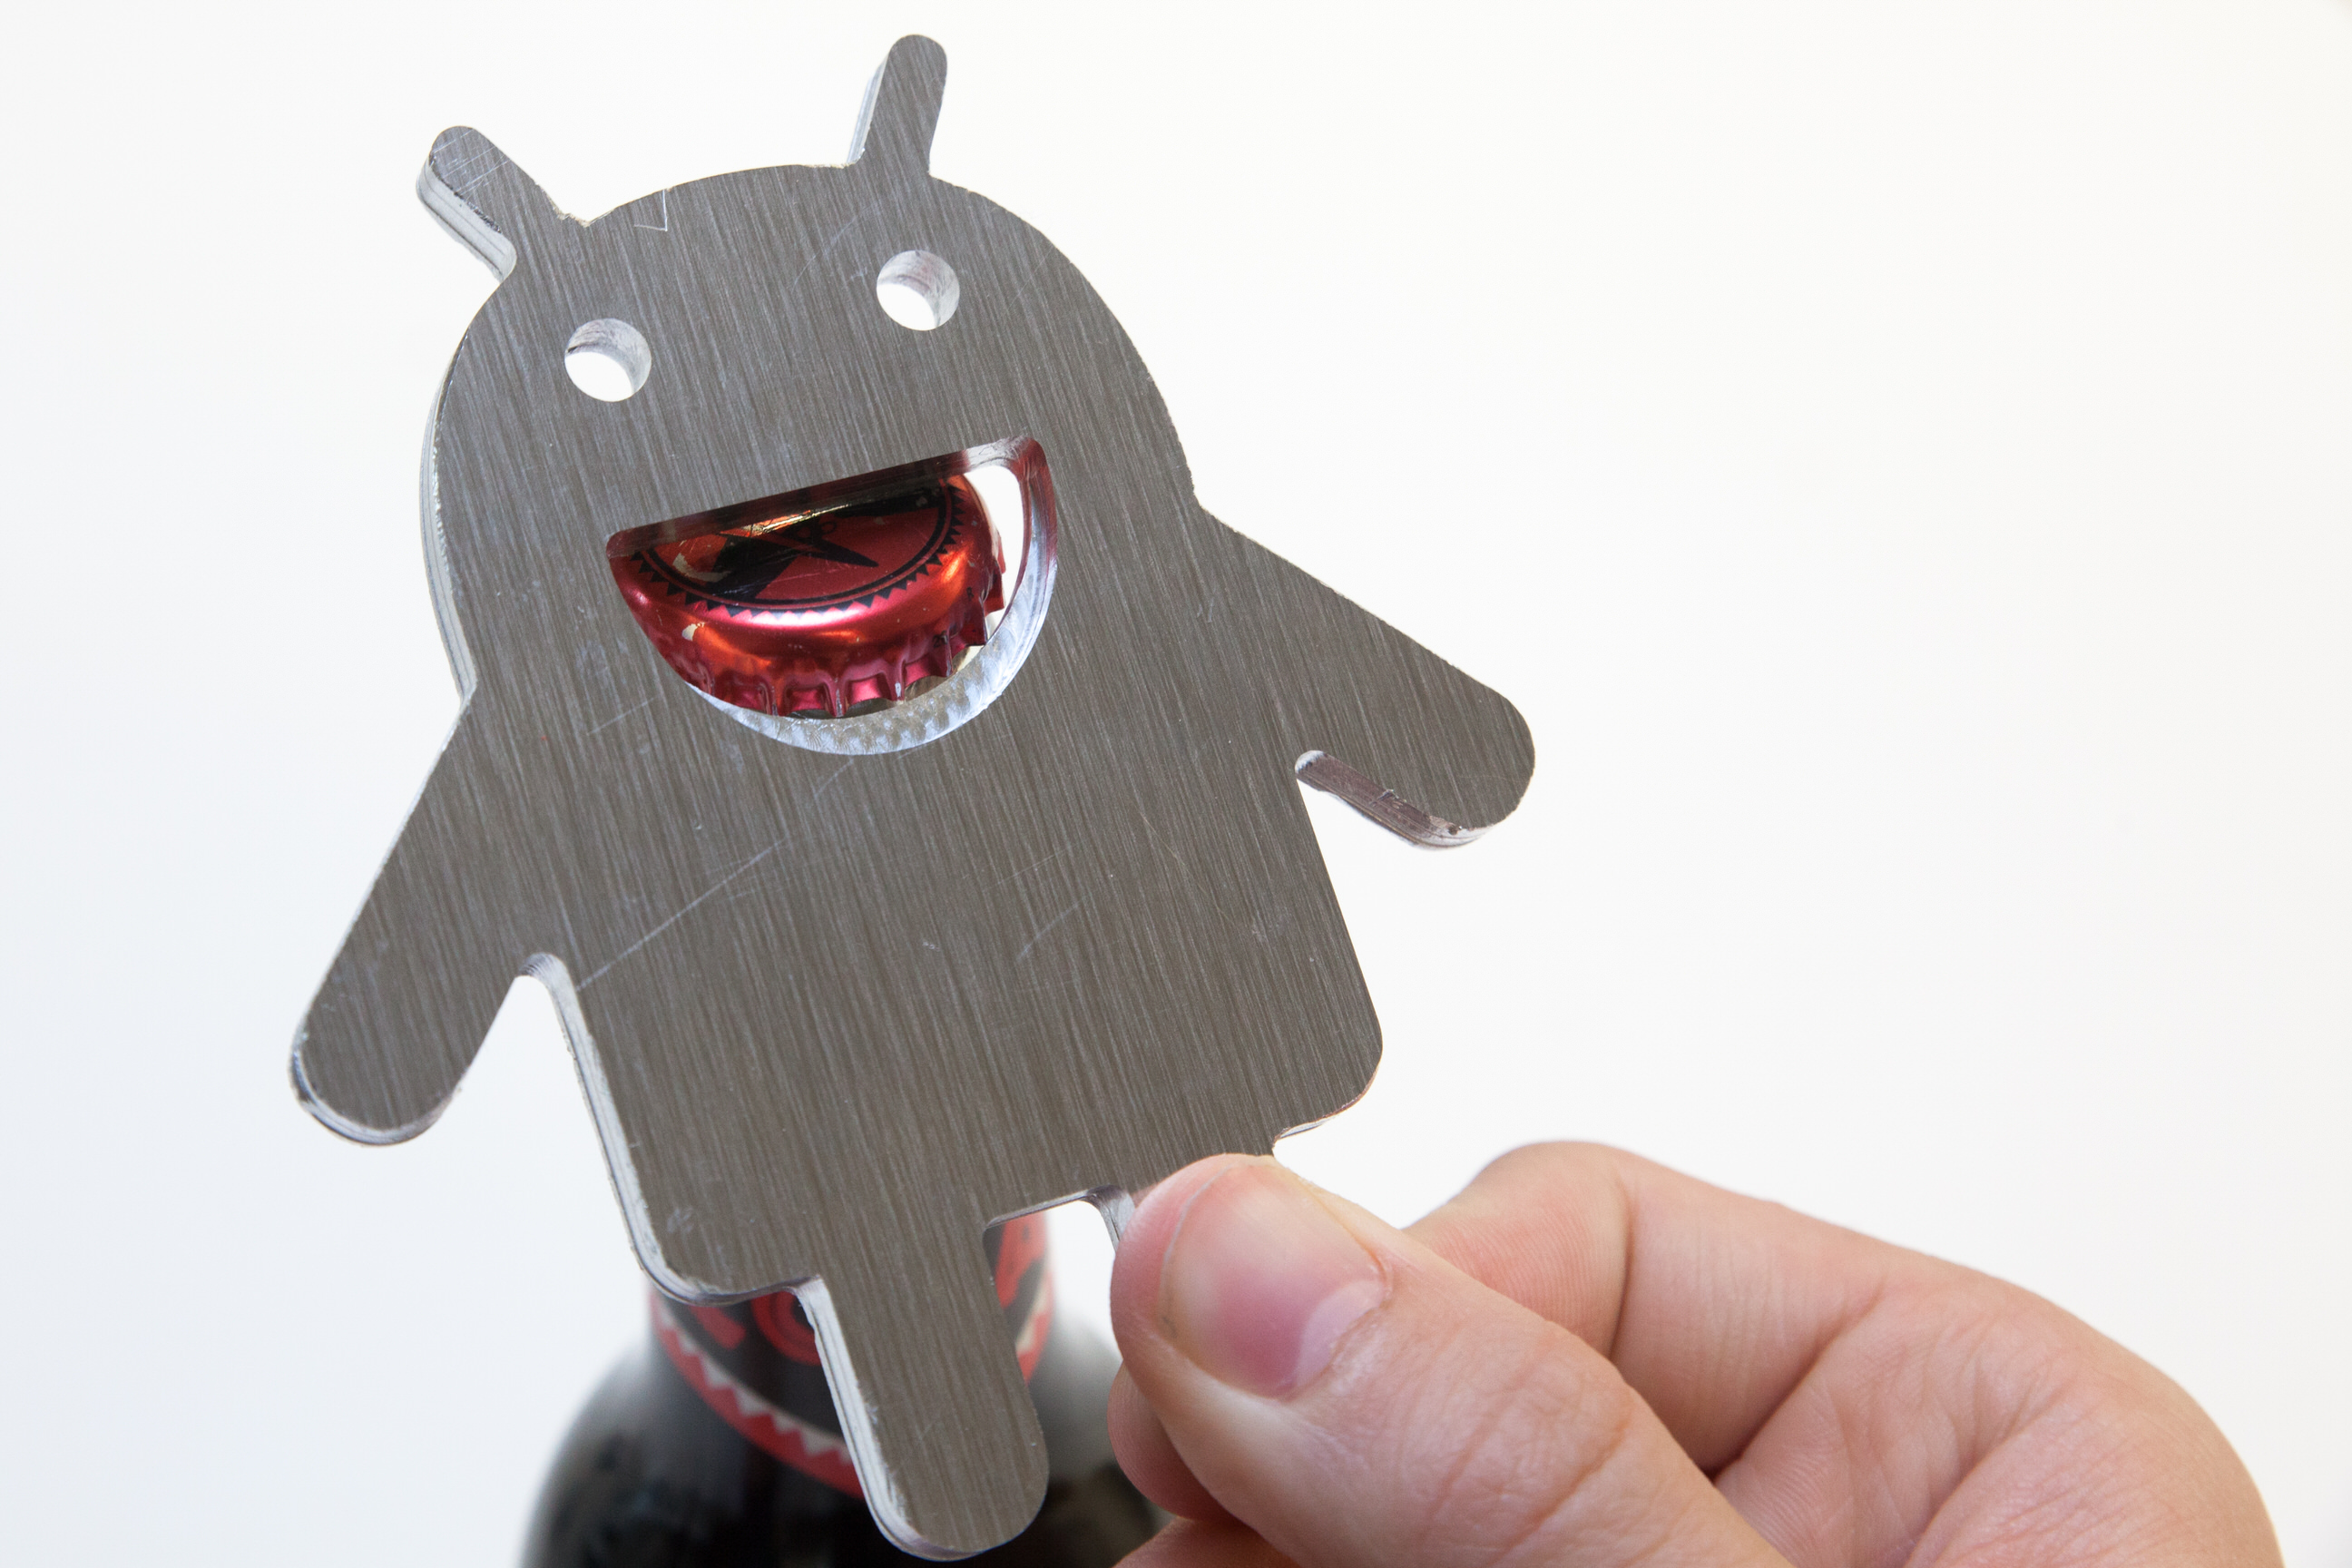
\includegraphics[height=0.6\textheight,width=\textwidth,keepaspectratio]{../img/fraese_flaschenoeffner.jpg}
    \end{center}
\end{frame}

\begin{frame}
    \frametitle{E-Werkstatt}
    % - gute Ausstattung
    % - Löten, Messen, Reparieren, Platinen bauen
    \begin{columns}[T]
        \begin{column}{0.55\textwidth}
            \begin{itemize}
                \item Platinenätzer, Multimeter, Lötkolben, Oszis, \dots
                \item Widerstände, Kondensatoren, Transistoren, \dots
                \item Für E-Techniker und solche, die es werden wollen
            \end{itemize}
        \end{column}
        \begin{column}{0.42\textwidth}
            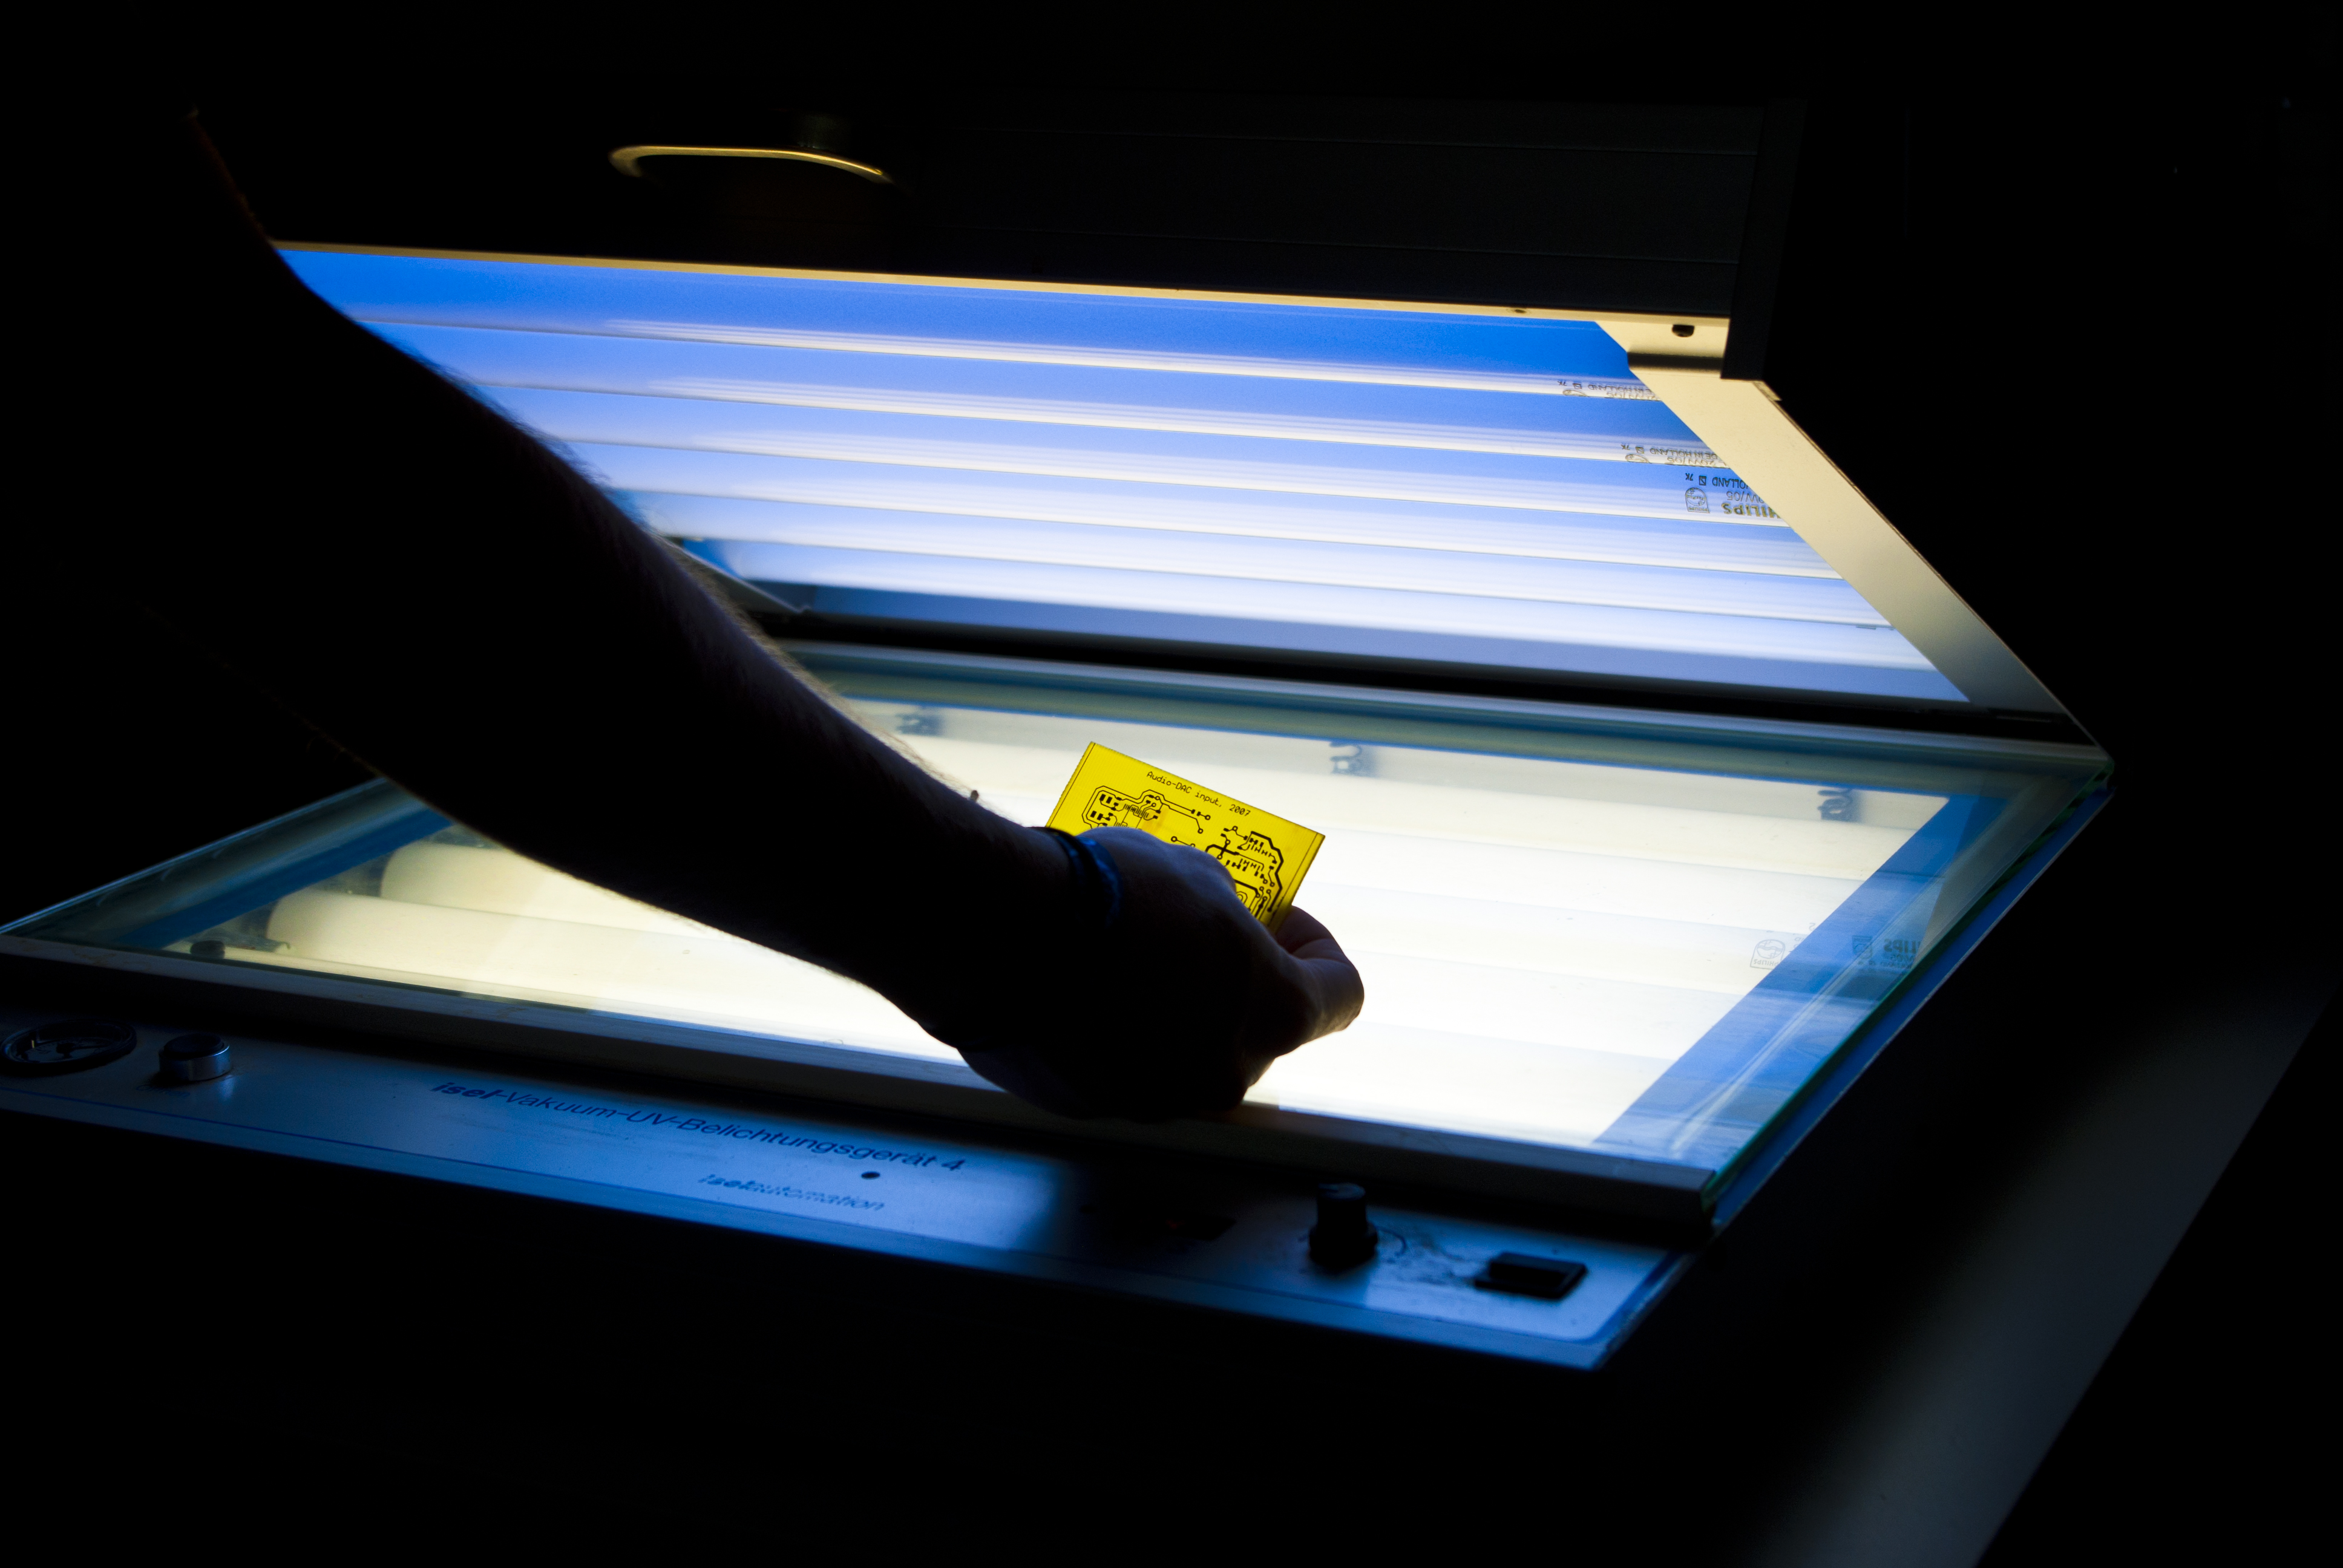
\includegraphics[width=\textwidth]{../img/belichten.jpg}
        \end{column}
    \end{columns}
\end{frame}

\begin{frame}
    \frametitle{\dots und vieles mehr}
    \begin{itemize}
        \item Druckluft und Fahrradwerkzeug
        \item Handwerkzeug
        \item Elektrowerkzeuge von Festool
        \item Nähmaschine, Stickmaschine, \dots
    \end{itemize}
\end{frame}

\begin{frame}
    \frametitle{Wo? Hinter den Hörsälen}
    % - sieht man sofort
    % - Türstatus
    \zweibilder[0.65\textheight]{../img/raumplan.pdf}{../img/fablab_door.jpg}
\end{frame}

\begin{frame}
    \frametitle{Wann? OpenLabs}
    % - Termine auf der Website
    % - ehrenamtliche Studierende
    % - Einweisungen, dann selbständig arbeiten
    Regelmäßige Öffnungszeiten auf unserem Kalender: {\color{blue} https://fablab.fau.de/termine}
    \begin{center}
        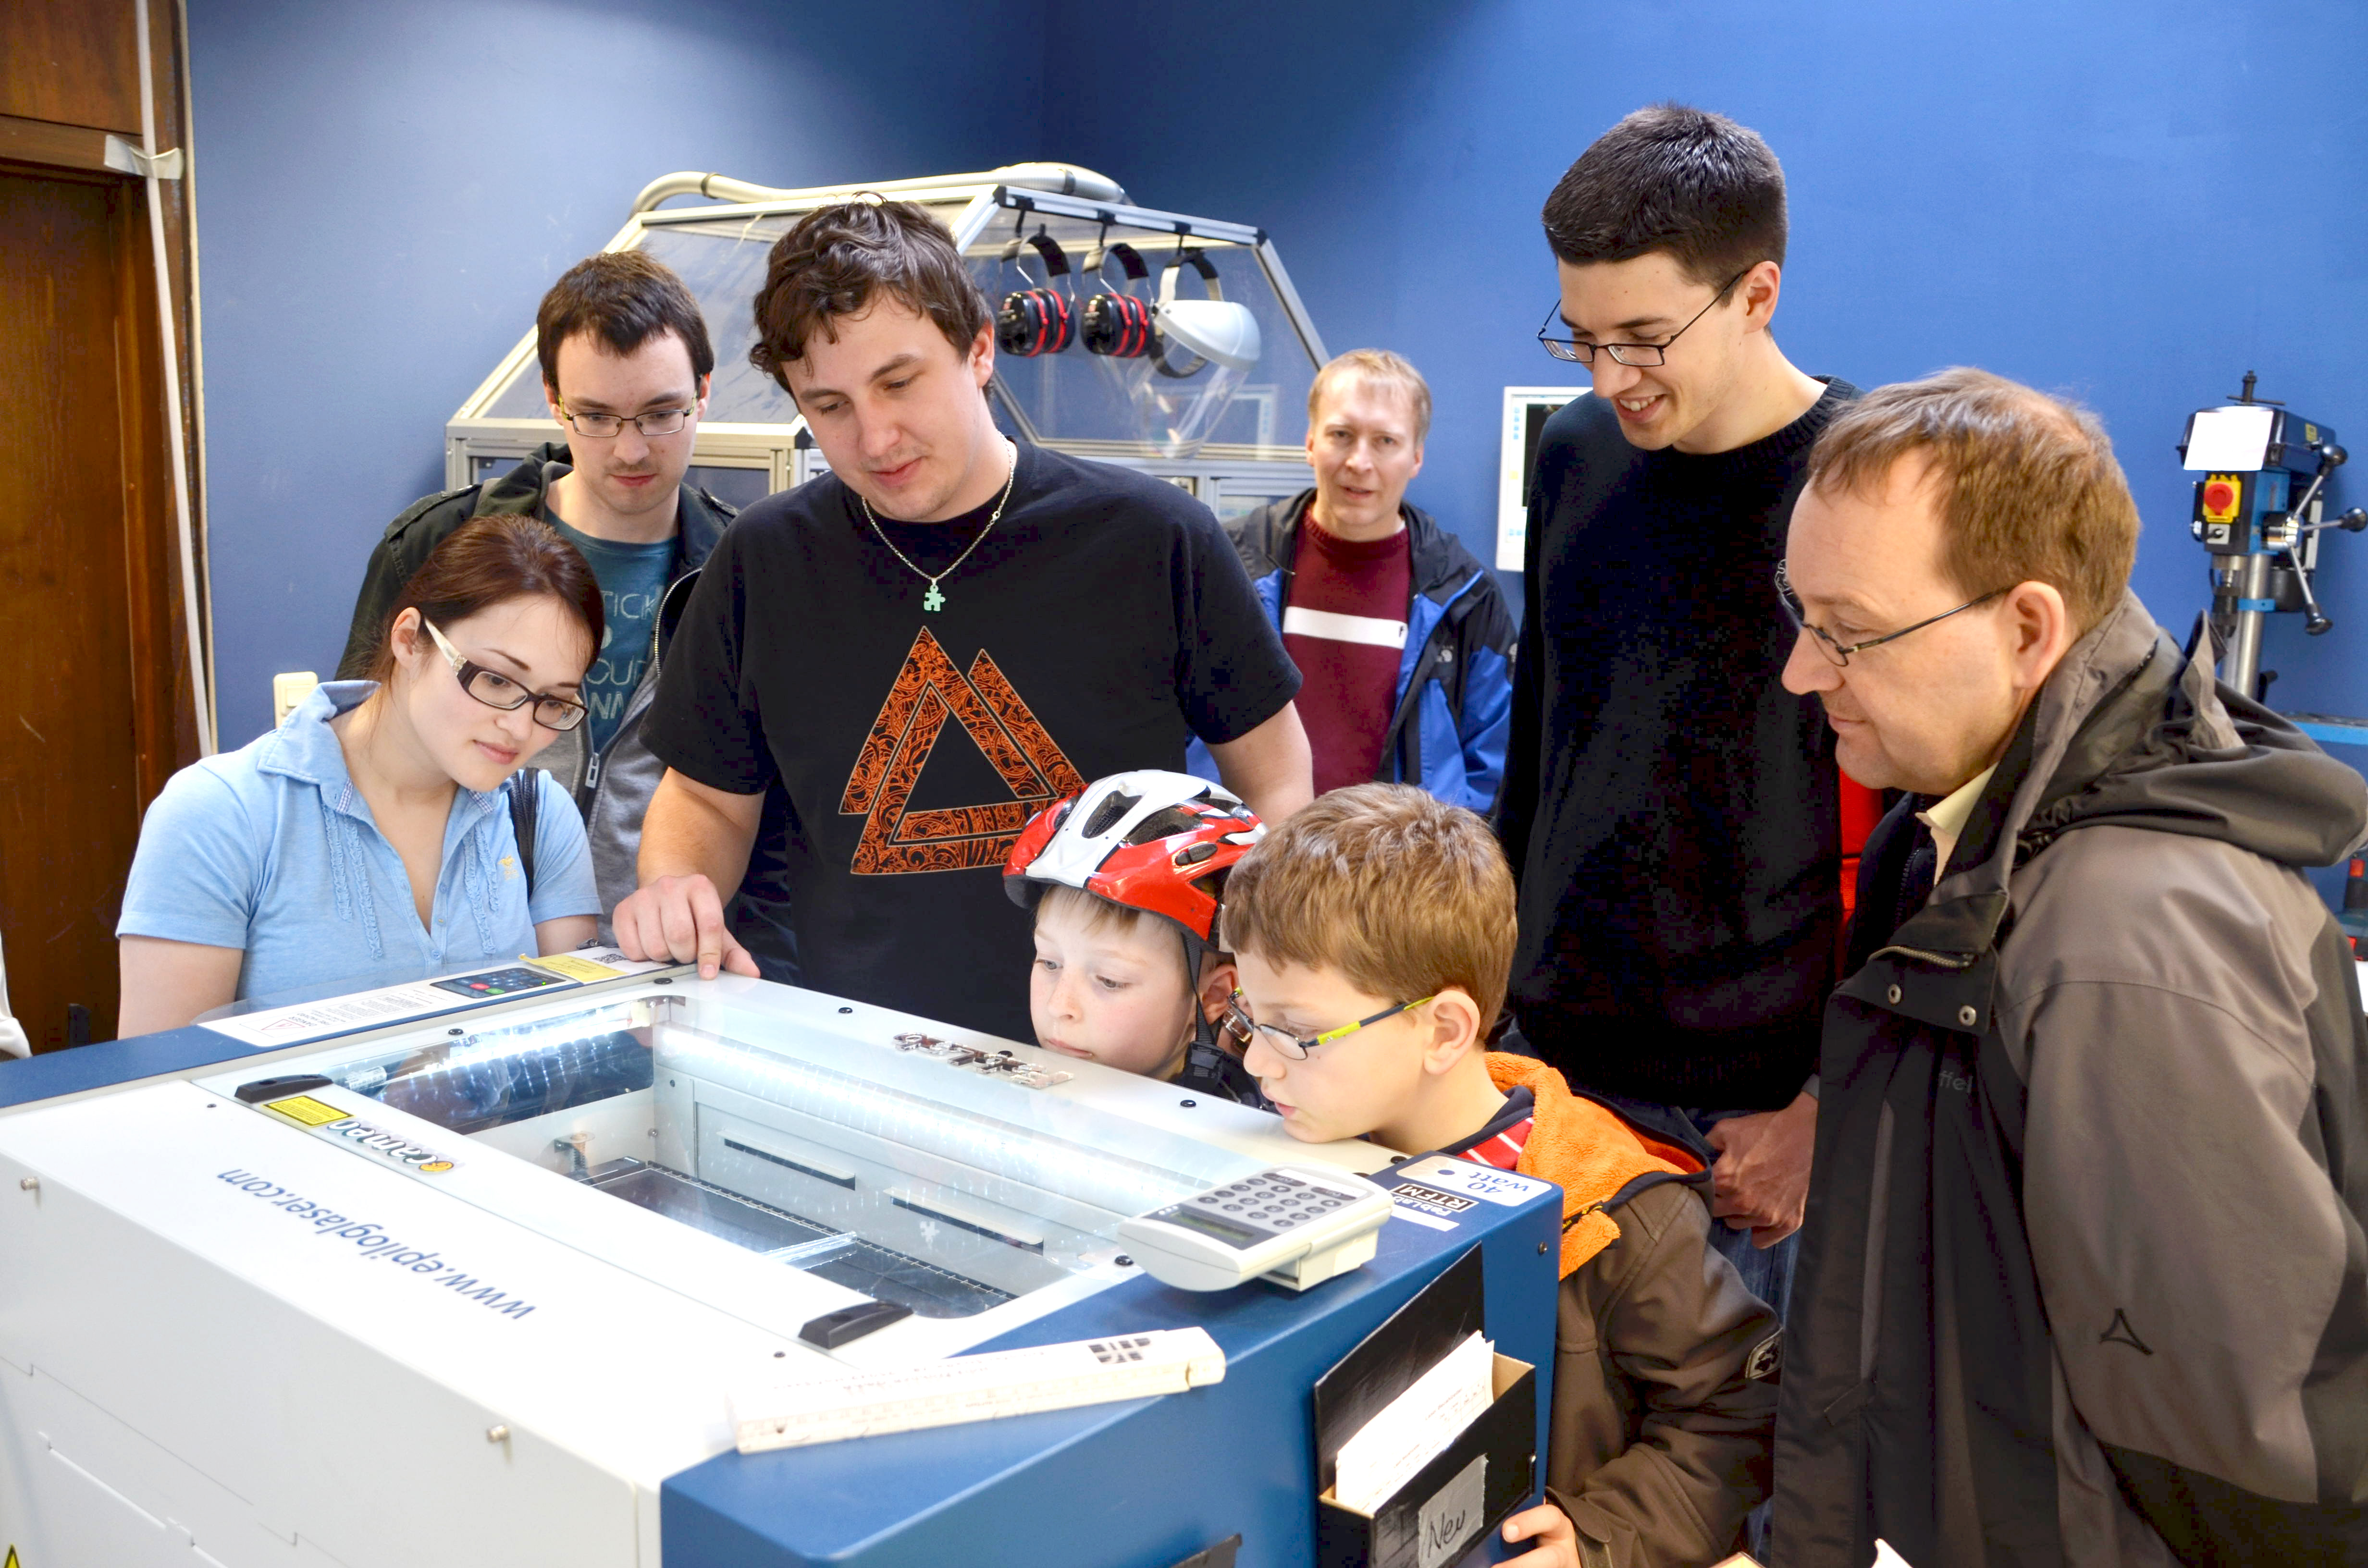
\includegraphics[height=0.55\textheight,width=\textwidth,keepaspectratio]{../img/einweisung.jpg}
    \end{center}
\end{frame}

\begin{frame}
    \frametitle{Warum ich? Komm vorbei, wenn du \dots}
    \begin{itemize}
        \item[] \dots wissen willst, was ein FabLab eigentlich ist
        \item[] \dots dir das Werkzeug für Projekte fehlt
        \item[] \dots mitmachen willst
        \item[] \dots dein Fahrrad aufpumpen musst
        \item[] \dots Langeweile zwischen Vorlesungen hast {\fontsize{16}{20}\selectfont -- oder dann besser nicht}
    \end{itemize}
\end{frame}

\begin{frame}[c]
    \begin{center}
        {\fontsize{44}{52}\selectfont\bfseries\color{fablabblue} fablab.fau.de}

        \bigskip
        
\includegraphics[height=0.45\textheight]{../img/qrcode_website.png}
    \end{center}
\end{frame}

\end{document}
